\section{\ce{[Cu(dca)_2(4-hydroxymethylpyridine)_2]_n}}
\subsection{Synthesis}
40 mL of aqua dest. were used to dissolve 0.48 g \ce{Cu(NO_3)_2*3 H_2O} (2 mmol), 0.36 g sodium dicyanamide (4 mmol) and 0.44 g 4-hydroxymethylpyridine (4 mmol). A two-hour stirring of the mixture was conducted at 70$^\circ$C. Before cooling it to room temperature, the blue solution was filtrated and stirred at the same temperature (15 minutes). After 24 hours blue plate-like crystals were obtained.
Anal. Calculated for \ce{C_{16}H_{14}CuN_{8}O_{2}} (413.90 g/mol): 46.43\% C; 3.41\% H; 27.07\% N;
Found: 46.31 \% C; 3.36\% H; 27.30 \% N;
IR (ATR, cm$^{-1}$): 3500(w), 2294(m), 2245 (m), 2170 (s), 1605 (s), 1566 (m), 1509 (w), 1426 (m), 1293 (m), 1205 (m), 1023 (s), 800 (m), 607 (w), 533 (m), 493 (w)

\begin{figure}[h!]
\centering
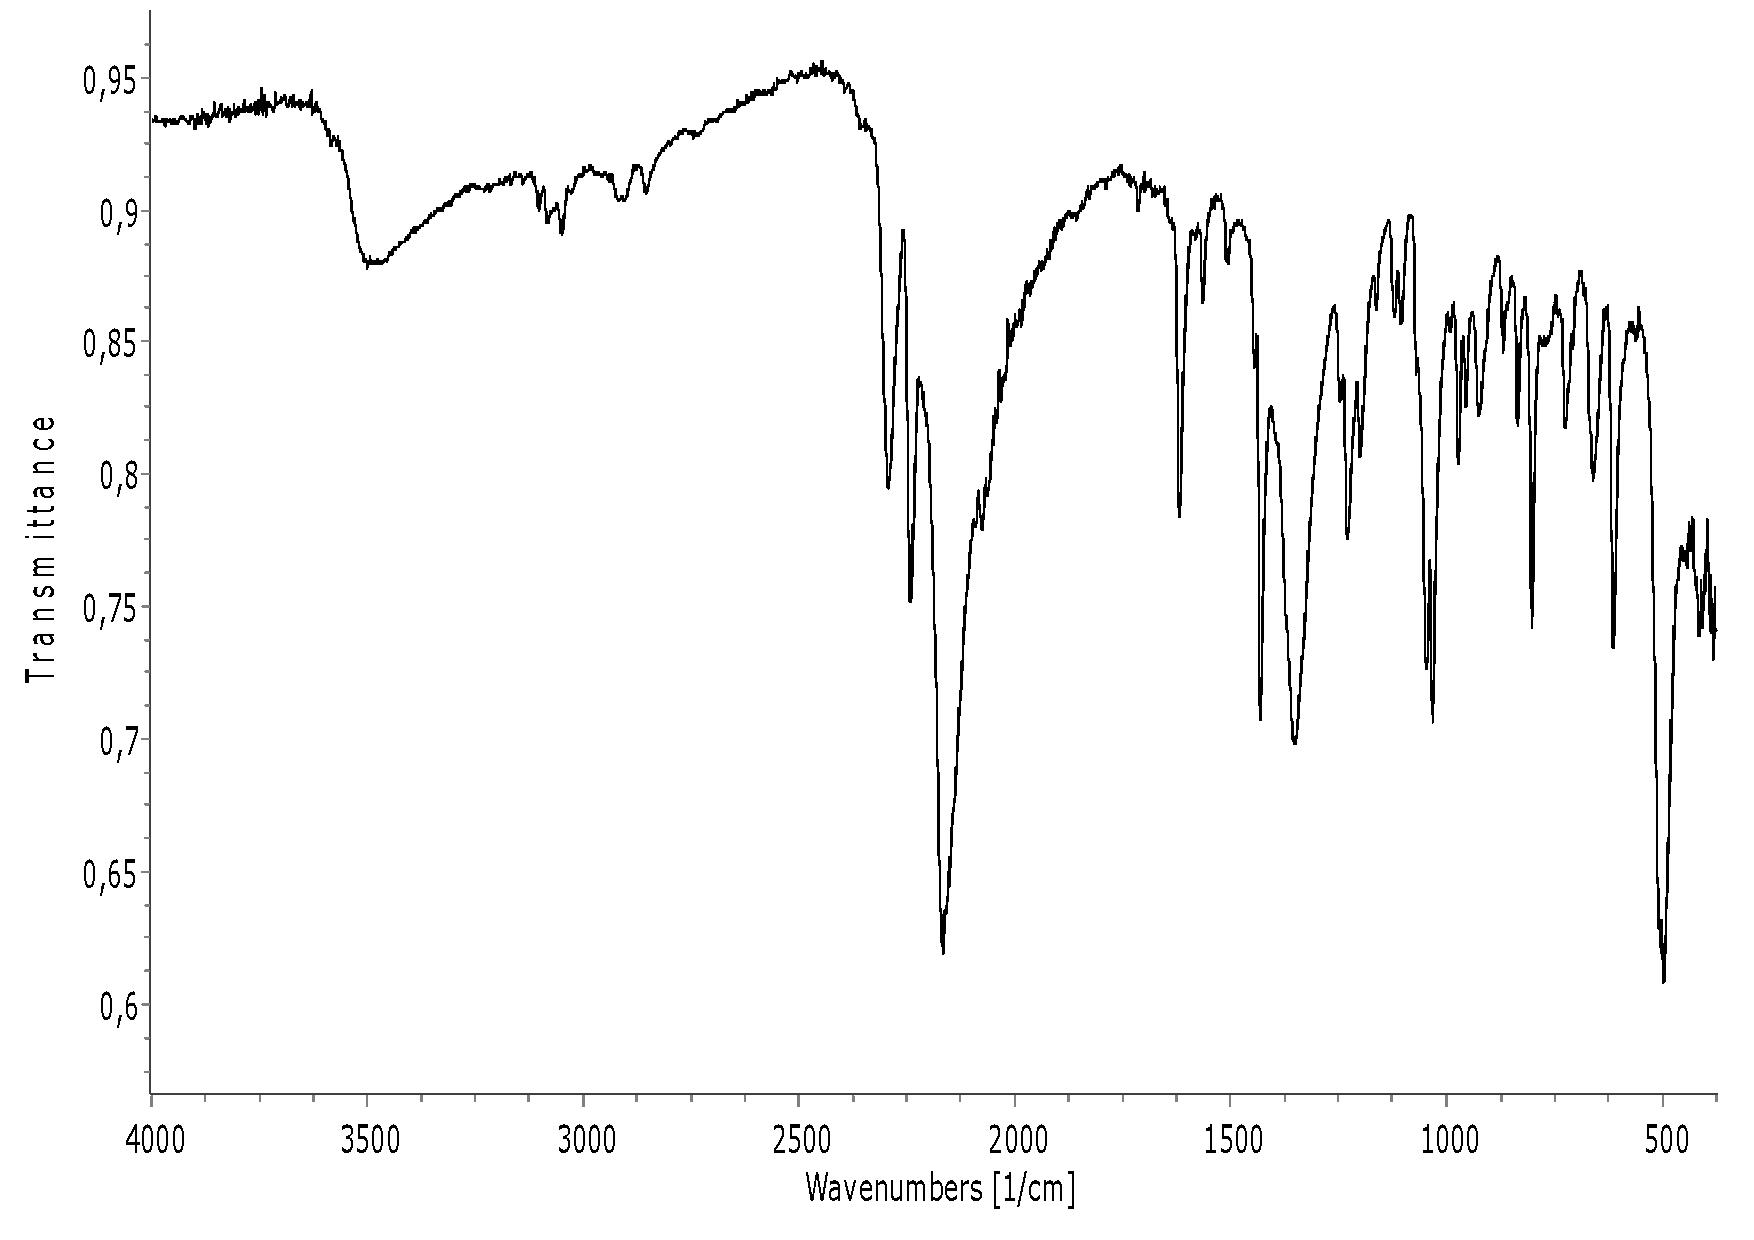
\includegraphics[width=1\textwidth]{figures/CuD4HOMP-IR.pdf}
\caption{IR spectrum of \ce{[Cu(dca)_2(4-HOMepy)_2]_n}}
\end{figure}


\subsection{Structural characterization}
Selected bond parameters of \ce{[Cu(dca)_2(4-HOMepy)_2]_n} are summarized in tab. \ref{batab:CuA4MOP}, a perspective view of a section of the polymeric chain is given in fig. \ref{fig:CuD4HOMP_pv} and a packing view in fig. \ref{fig:CuD4HOMP_packv}.  The Cu(1) is located on an inversion center. This metal cation is coordinated by pyridine N donor atom of two 4-methanolpyridine molecules in trans configuration and four N atoms of dicyanamide anions. The latter act in the bis-$\mu$(1,5)-bridging mode to generate polymeric chains of polyhedra oriented along the c-axis of the monoclinic unit cell. The \ce{CuN6} chromophore possesses an elongated square bipyramidal geometry, with short Cu(1)-N(1) and Cu(1)-N(2) bond distances of 2.014(4) and 1.990(4) \AA, respectively. Its semi-coordinative Cu(1)-N(4b,c) bond distances equals 2.488(5) \AA. The asymmetric dicyanamide bridges have the following bond parameters: Cu-N-C: 171.1(4) and 134.0(5)$^\circ$; N-C-N: 174.8(6) and 174.1(7)$^\circ$; C-N-C: 121.1(5)$^\circ$; C-N(nitril) 1.148(7) and 1.147(7) \AA; C-N(amide): 1.299(7) and 1.302(7) \AA. The intra-chain Cu...Cu distance of 7.2754(12) \AA is similar to the shortest inter-chain metal..metal separation of 7.2432(12) \AA. The hydroxy-group of the pyridine derivative ligand forms hydrogen bond of type O-H\ce{***}N to N(3) and N(4) atom of adjacent dicyanamide anions. This generates a 3D supramolecular network system (O(1)-H(90)\ce{***}N(3\#1) = 124(5)$^\circ$, O(1)\ce{***}N(3\#1) = 3.199(8) \AA; [O(1)-H(90)\ce{***}N(4\#2) = 141(6)$^\circ$, O(1)\ce{***}N(4\#2) = 3.101(7) \AA (\#1): 1+x,y,z]; (\#2): 1+x,1/2-y,-1/2+z).

\renewcommand{\arraystretch}{1.1}
\begin{table}[htpb!]
\centering
\captionabove{Selected bond lengths (\AA) and angles ($^\circ$) for \ce{[Cu(dca)_2(4-HOMepy)_2]_n};Symmetry codes: (a) -x,1-y,-z; (b) -x,1-y,1-z; (c) x,y,-1+z; (d) x,y,1+z; (e) -x,1-y,-1-z.}
\begin{tabular}{|l|l|l|l|}
\hline
Cu(1)-N(1a) & 2.014(4) & Cu(1)-N(4b) & 2.488(5)\\
\hline
Cu(1)-N(2a) & 2.1990(4)& N(3)-C(7) & 1.299(7)\\
\hline
N(2)-C(7) & 1.148(7) & N(3)-C(8) & 1.302(7)\\
\hline
N(4)-C(8) & 1.147(7) &  & \\
\hline
\hline
N(2)-Cu(1)-N(1) & 90.51(17) & N(2a)-Cu(1)-N(1a) & 91.16(17)\\
\hline
N(4)-Cu(1)-N(1a) & 90.37(17) & N(2)-Cu(1)-N(2a) & 180.0\\
\hline
Cu(1)-N(2)-C(7) & 171.1(4) & N(2)-C(7)-N(3) & 174.8(6)\\
\hline
Cu(1)-N(4)-C(8)& 134.0(5) &N(4)-C(8)-N(3) & 174.1(7)\\
\hline
C(7)-N(3)-C(8)& 121.1(5) & &\\
\hline
\end{tabular}
\label{batab:CuA4MOP}
\end{table}


\begin{figure}[htpb!]
\centering
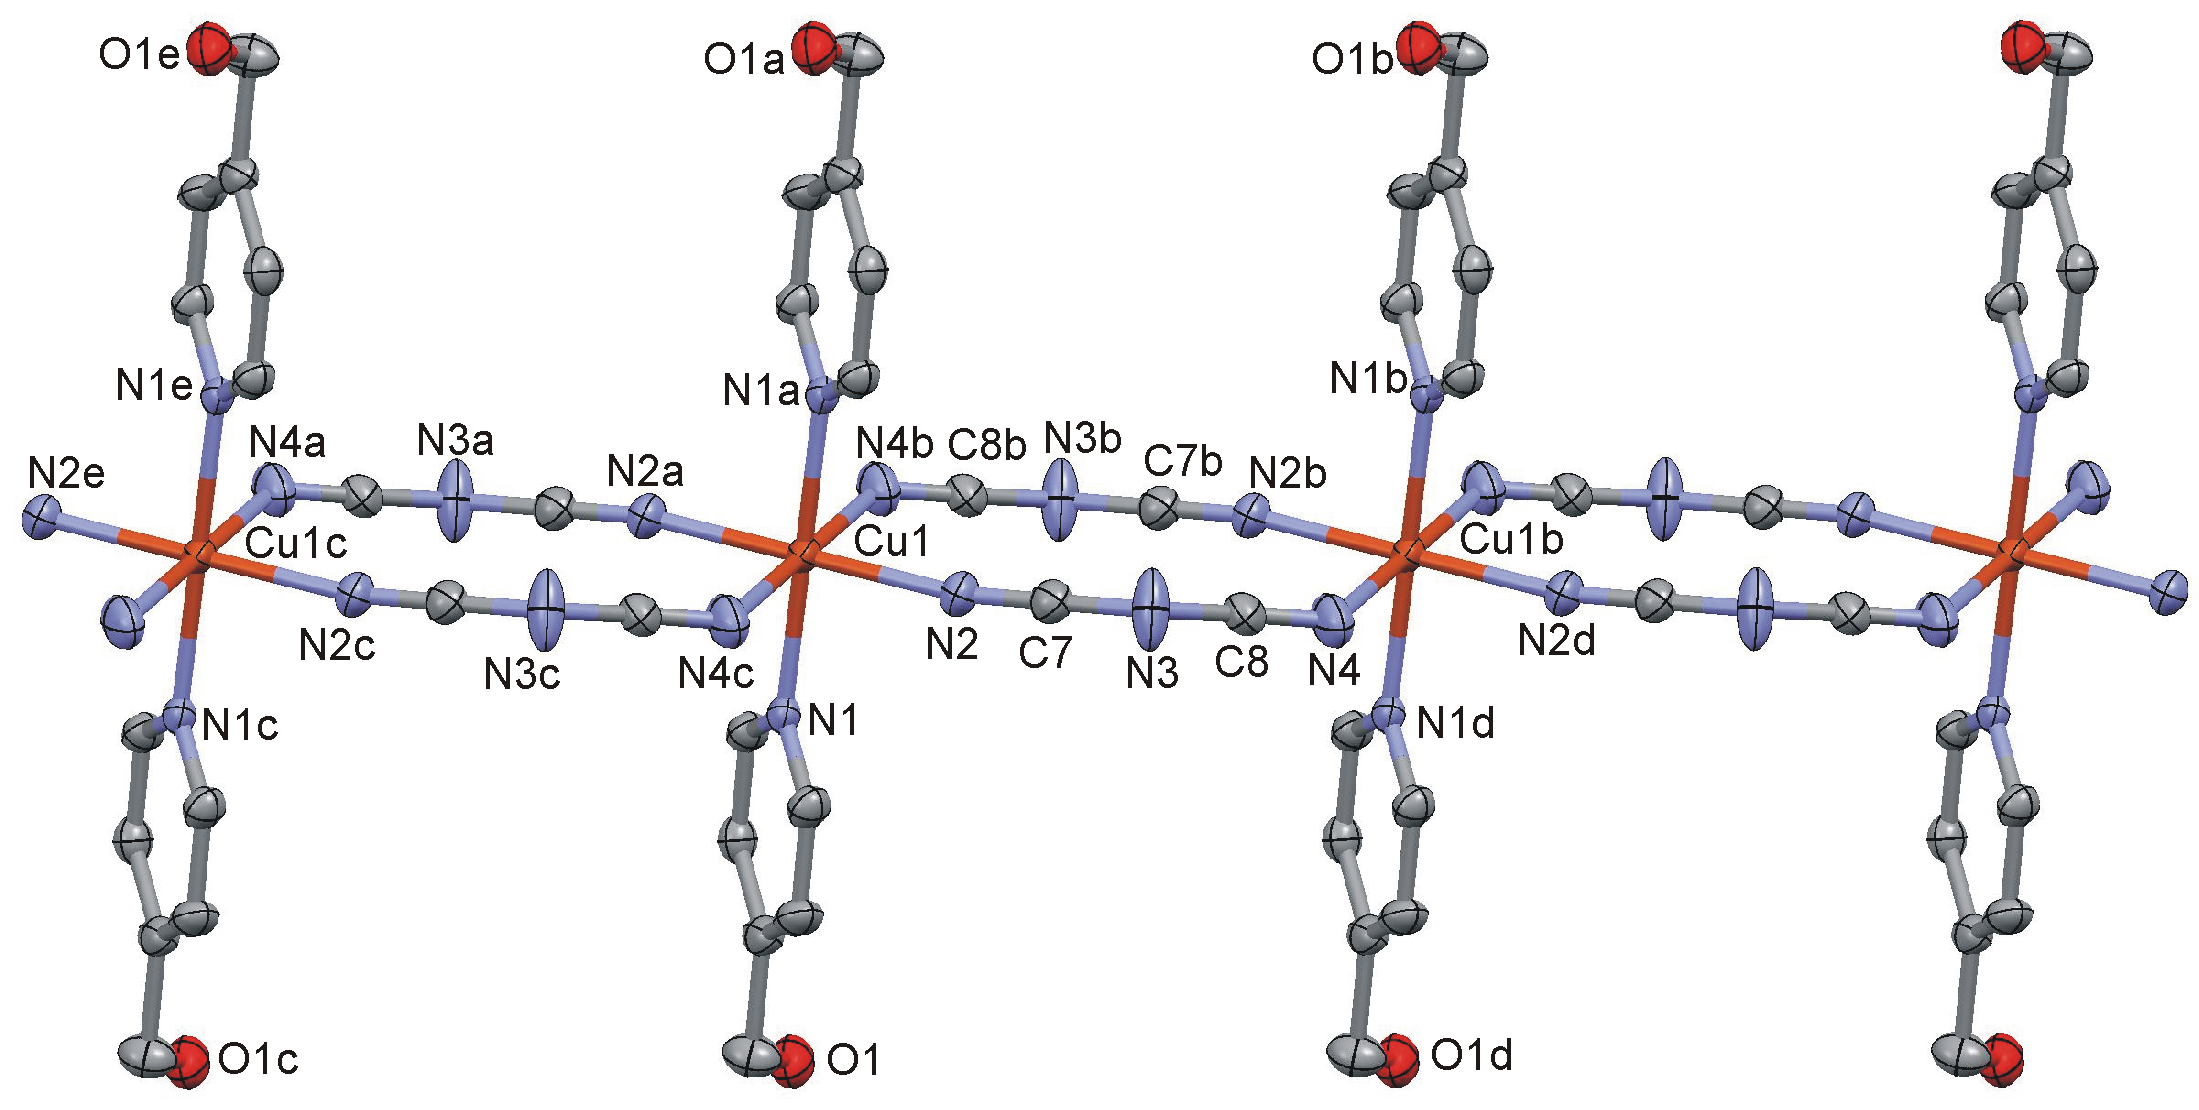
\includegraphics[width=1\textwidth]{figures/CuD_4OMP_FIGm11.png}
\caption[Perspective view of \ce{[Cu(dca)_2(4-HOMepy)_2]_n}]{Perspective view of a section of the polymeric chain of \ce{[Cu(dca)_2(4-HOMepy)_2]_n} together with the atom numbering scheme. Symmetry codes: (a) -x,1-y,-z; (b) -x,1-y,1-z; (c) x,y,-1+z; (d) x,y,1+z; (e) -x,1-y,-1-z.}
\label{fig:CuD4HOMP_pv}
\vspace{\floatsep}
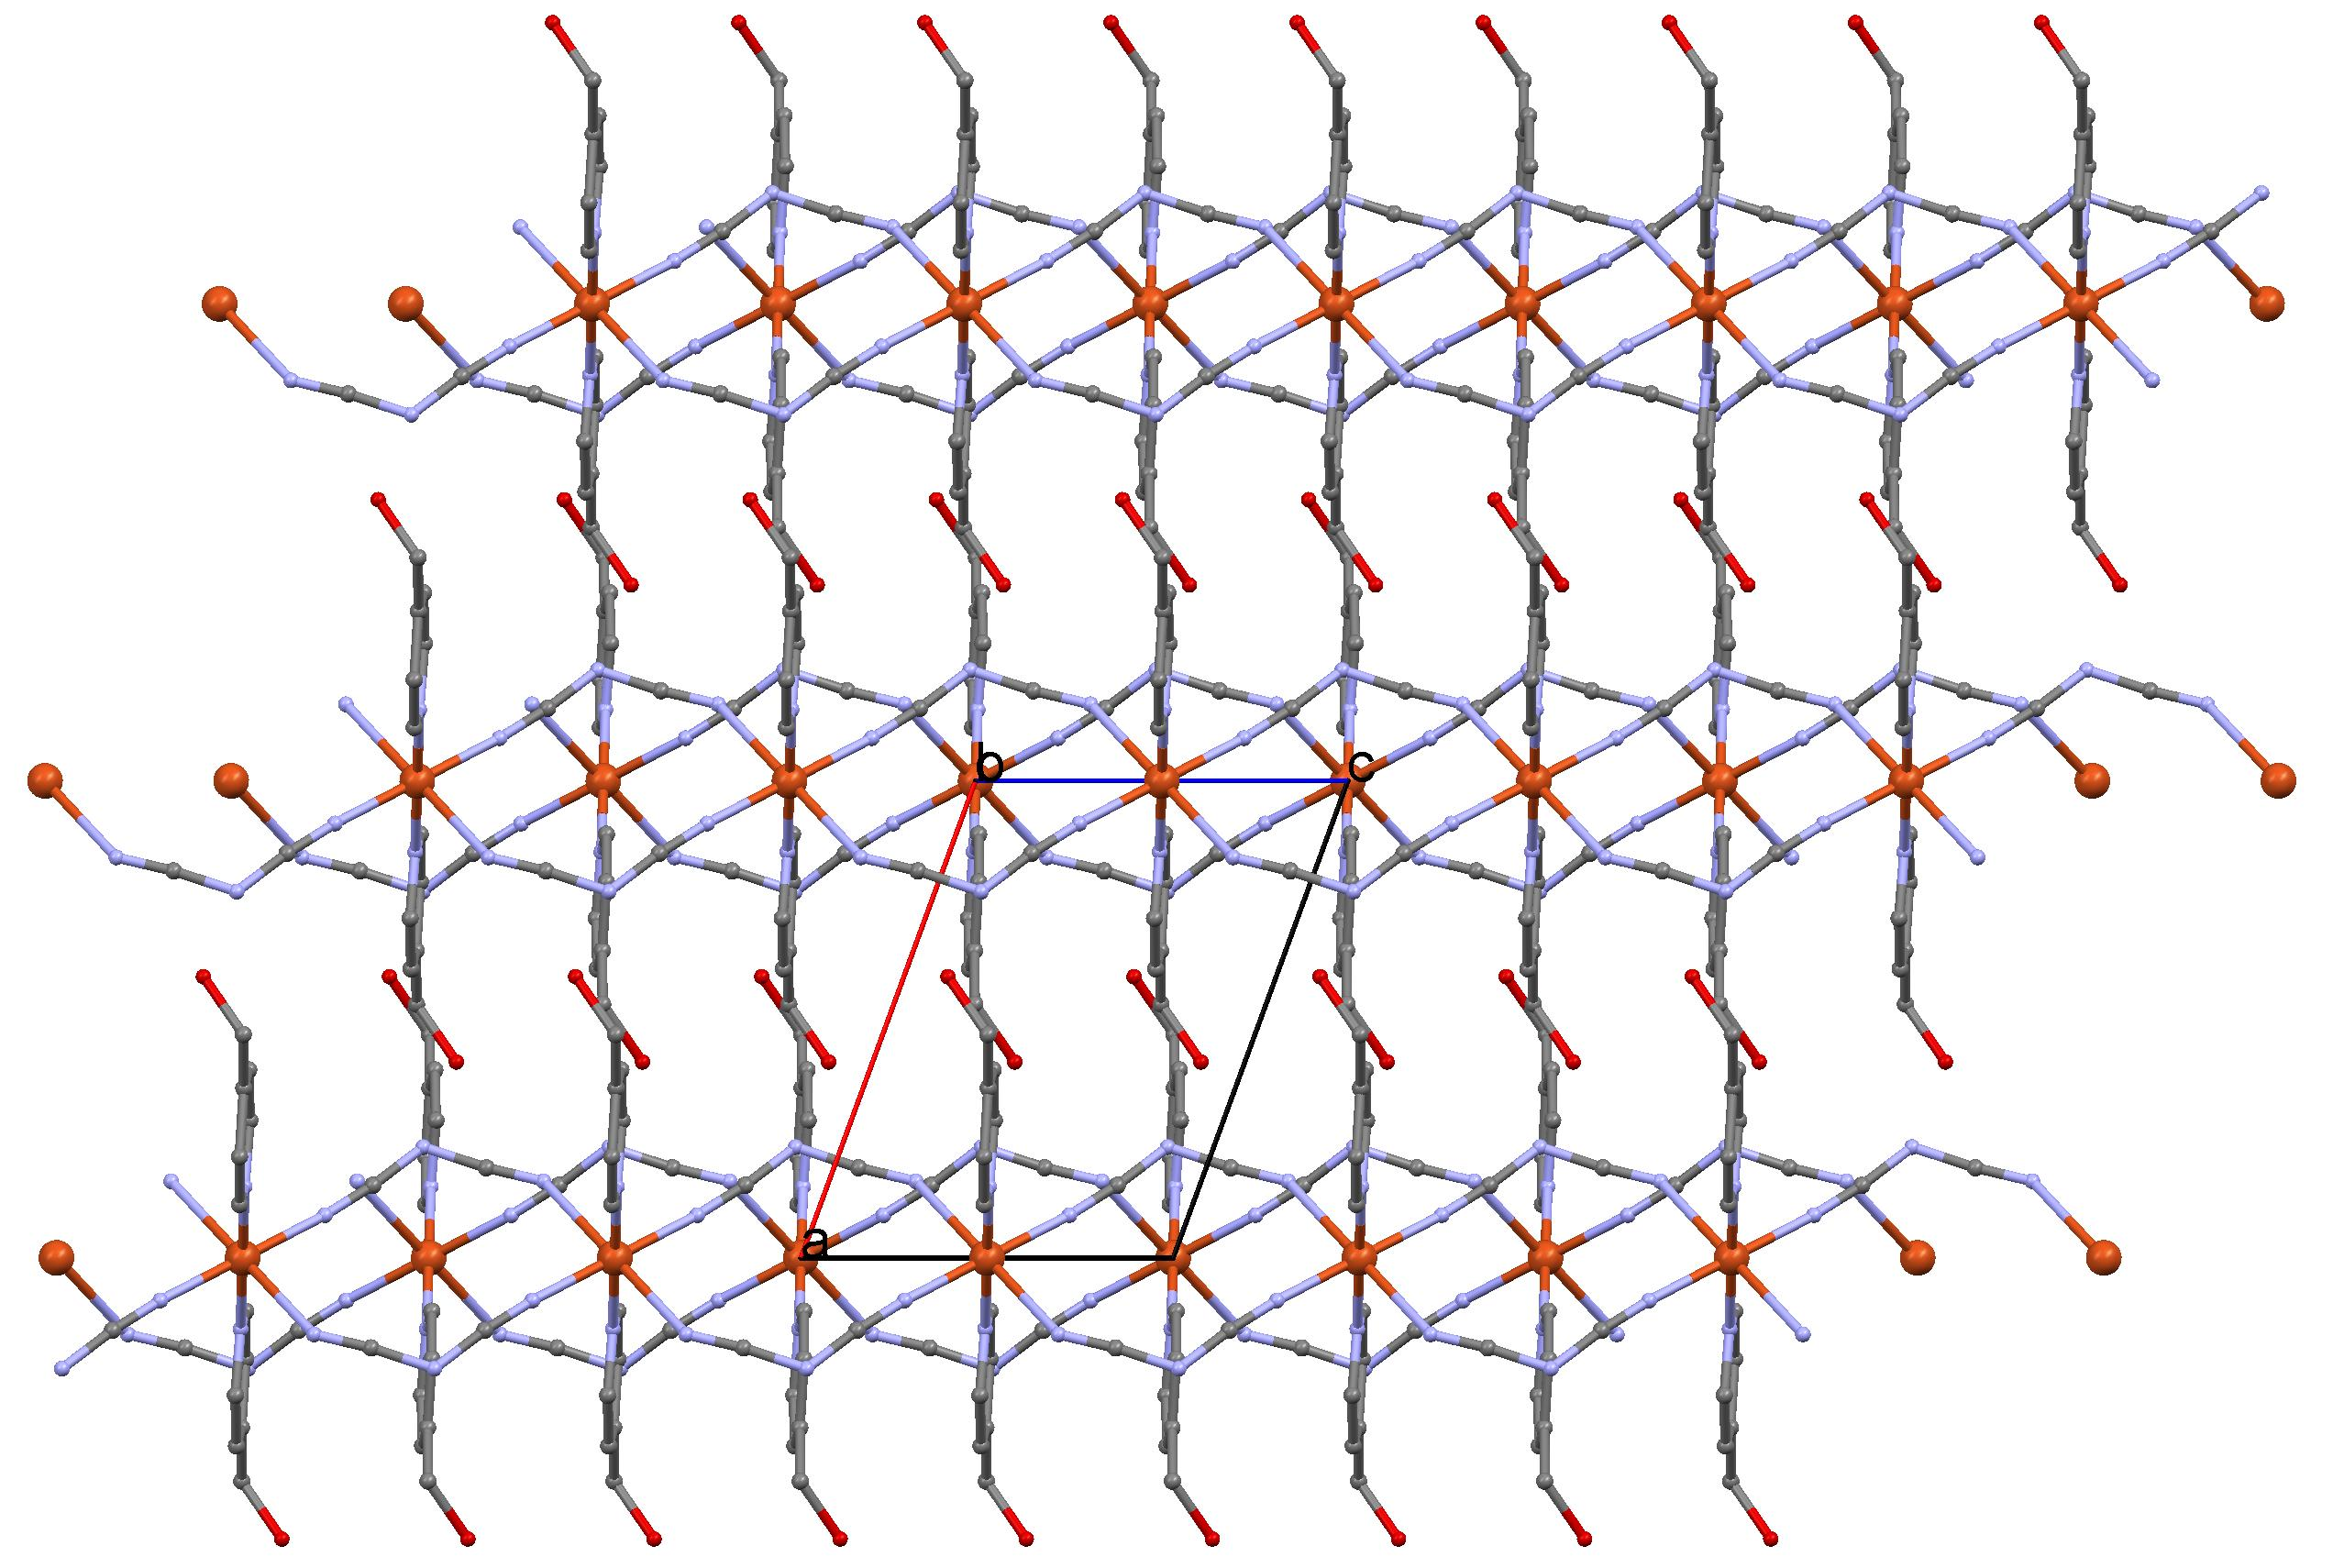
\includegraphics[width=1\textwidth]{figures/cud_4omp_CB.png}
\caption{Packing plot of \ce{[Cu(dca)_2(4-HOMepy)_2]_n}}
\label{fig:CuD4HOMP_packv}
\end{figure}

\renewcommand{\arraystretch}{1.5}
\begin{table}
\centering
\captionabove{Crystallographic data and processing parameter of \ce{[Cu(dca)_2(4-HOMepy)_2]_n}}
\begin{tabular}{ | l |  l | }
\hline
Empirical formula & \ce{C_{16}H_{14}CuN_{8}O_{2}}\\
\hline
Formula mass & 413.90\\
\hline
System & monoclinic\\
\hline
Space group & P2$_1$/c\\
\hline
a ({\AA}) & 9.9292(14)\\
\hline
b ({\AA}) & 12.527(2)\\
\hline
c ({\AA}) & 7.2754(12)\\
\hline
$\alpha$ ($^\circ$) & 90\\
\hline
$\beta$ ($^\circ$) & 110.109(7)\\
\hline
$\gamma$ ($^\circ$) & 90\\
\hline
V (\AA$^{3}) $  & 849.8(2)\\
\hline
Z & 2\\
\hline
T (K) & 100(2)\\
\hline
$\mu$ (mm$^{-1}$) & 1.317\\
\hline
 D$_{calc}$ (Mg/m$^{3}$) & 1.618\\
\hline
Crystal size (mm) & 0.41 x 0.26 x 0.05\\
\hline
$\theta$ max ($^\circ$) & 26.35\\
\hline
Data collected & 6328\\
\hline
Unique refl./ R$_{int}$ & 1728 / 0.0533\\
\hline
Parameters & 127\\
\hline
Goodness-of-Fit on F$^{2}$ & 1.337\\
\hline
R1 / wR2 (all data) & 0.0743/0.1685\\
\hline
Residual extrema (e/\AA$^{3}$) & 1.26 /-0.95\\
\hline
\end{tabular}

\label{ptab:CuD4HOMP}

\end{table}



